
\section{Infrastruktur}
\label{Infrastruktur}

\subsection{Continuous Integration}
\label{Infrastruktur:Continuous Integration}

In unserem Projekt wird \ac{CI} einerseits für das automatische Erstellen dieser Dokumentation mit LaTeX verwendet und andererseits, um automatische Tests für die Implementation auszuführen.
Beides wird im Folgenden kurz beschrieben.

\subsubsection{Erstellen der LaTeX-Dokumentation}
\label{CI:Erstellen der LaTeX-Dokumentation}

Bei jedem Git Commit in das Repository der Dokumentation~\cite{github:thesis} wird mit Continuous Integration ein PDF erstellt.
So wird sichergestellt, dass die Dokumentation keine syntaktischen Fehler aufweist.
Das PDF wird in unser internes JIRA hochgeladen und direkt dem Task angehängt, der zum Branch gehört.

Für diese Continuous Integration haben wir uns für Travis CI ~\cite{travis-ci} entschieden, da die Integration mit Github gut funktioniert und das Produkt für Open-Source-Projekte kostenlos ist.
Allerdings bietet Travis \acs{CI} keine direkte Unterstützung für eine LaTeX-Umgebung an. Die LaTeX-Pakete aus den Repositories sind ausserdem veraltet.
So muss bei jedem Build die LaTeX-Umgebung kompiliert werden, damit immer die neueste Version aller Pakete verwendet werden kann.


\subsubsection{CI für die Unit Tests}
\label{CI:CI für Backend}

Für die Continuous Integration der Web-Applikation braucht es eine Umgebung mit Node JS, um die Applikation zu kompilieren und die Tests auszuführen.
Für den \nameref{Implementation:ÖV-Güteklassen 2018 Generator} wird eine entsprechende Umgebung für Python benötigt.
Dazu bietet sich ebenfalls Travis \acs{CI}~\cite{travis-ci} an.
Die entsprechenden Umgebungen sind bereits vorhanden, womit der Konfigurationsaufwand sehr klein bleibt.
Ebenfalls existiert ein Cron-Job, welcher die Builds und somit die Tests in regelmässigen Abständen ausführt.

\subsection{Deployment}
\label{Infrastruktur:Deployment}

Für das Deployment wurde eine Docker-Umgebung eingerichtet, die für die einfache Handhabung der Berechnung der \gls{ÖV-Güteklassen} 2018 dient.
Die Details dazu sind im Kapitel \ref{Implementation:ÖV-Güteklassen 2018 Generator} beschrieben.

Um die berechneten \gls{ÖV-Güteklassen} in der Web-Applikation zu visualisieren, wurde eine zusätzliche Docker-Umgebung vorbereitet.
Diese kombiniert die Web-App, Backend sowie der Tile-Server, damit man die komplette Applikation ohne zusätzliche Konfiguration lokal oder auf einem Server deployen kann.
Dies hat den Vorteil, dass das Setup, welches deployed wird, analog lokal gestartet und getestet werden kann.
Um die Services in einem gemeinsamen Endpoint zu verbinden, wird eine Nginx-Instanz als Reverse-Proxy verwendet, der die \acs{API}-Requests an die entsprechenden Endpoints weiterleitet.
Die Umgebung ist in Abbildung \ref{fig:deployment_web-app} dargestellt.

\begin{figure}[ht]
    \centering
    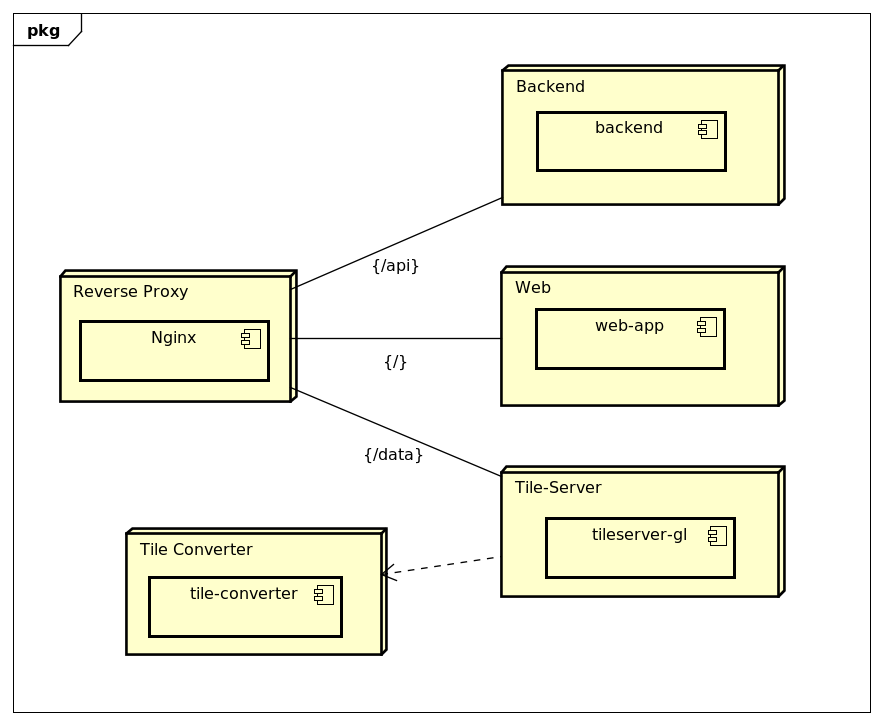
\includegraphics[width=0.8\linewidth]{projectdoc/img/deployment_web-app}
    \caption[Deployment-Diagramm der Web-Applikation]{Deployment-Diagramm der Web-Applikation mit den entsprechenden Backend-Services}
    \label{fig:deployment_web-app}
\end{figure}

Zusätzlich wurde ein Service eingerichtet, um die errechneten \gls{ÖV-Güteklassen} im \gls{GeoJSON}-Format in Map-Tiles, sprich in MBTiles (siehe Kapitel \ref{Implementation:Tile-Converter}) umzuwandeln, damit der Tile-Server damit umgehen kann.
Der Benutzer kann die \gls{GeoJSON}-Dateien in einem Ordner ablegen und die Docker-Umgebung mit Docker Compose starten.
Die Aufbereitung der Map-Tiles geschieht dann automatisch im Hintergrund.

\subsection{Version Control}
\label{Infrastruktur:Version Control}

Alle Artefakte, welche in dieser Arbeit erstellt wurden, sind öffentlich auf Github verfügbar.
Es wurde dazu eine Github Organisation mit dem Namen "`public-transport-quality-grades"'~\cite{github} erstellt.

In der Tabelle \ref{table:github_overview} sind die einzelnen Repositoriers aufgelistet und kurz der Inhalt erläutert.
Diese soll als Übersicht dienen und einen raschen Einstieg in die Version Control ermöglichen.

\begin{table}[H]
    \begin{tabular}{l p{10.6cm}}
        \toprule
        \textbf{Name}           & \textbf{Inhalt}\\
        \midrule
        thesis~\cite{github:thesis}
                                & Bachelorarbeit\\
        oevgk18-specification~\cite{github:oevgk18-specification}
                                & Aus der Bachelorarbeit extrahierte \gls{ÖV-Güteklassen} 2018 Spezifikation\\
        oevgk18-generator~\cite{github:oevgk18-generator}
                                & \gls{ÖV-Güteklassen} 2018 Generator\\
        web-app~\cite{github:web-app}
                                & Web-Applikation zur Visualisierung der \gls{ÖV-Güteklassen} 2018\\
        backend~\cite{github:backend}
                                & Backend der \gls{ÖV-Güteklassen} 2018\\
        backend-api~\cite{github:backend-api}
                                & Dokumentation des Web-\acs{API} des Backend\\
        admin~\cite{github:admin}
                                & Sitzungsprotokolle und Entscheidungen\\
        infrastructure~\cite{github:infrastructure}
                                & Interne Projekt-Infrastruktur (Jira-Setup, \dots)\\  
        playground~\cite{github:playground}
                                & Spielwiese für die Evaluation von Frameworks\\
                                
        \bottomrule
    \end{tabular}
    \caption{Github Repository Übersicht}
    \label{table:github_overview}
\end{table}